\hspace{1.25cm}Прежде чем запускать приложение необходимо настроить локальный сервер Apache. Подробную инструкцию по установке и настройке Apache вы можете увидить здесь: 
http://www.webbcare.org/lectures/web-servers/Lecture15.pdf.

Можно также воспользовать уже настроенными пакетами, такими как xampp (https://www.apachefriends.org/ru/index.html) или denver \\
(http://www.denwer.ru/). 
Файлы, при распаковке, следует поместить в папку htdocs (все скрипты, запускаемые на локальной машине
по умолчанию, находятся в данной папке) в уже настроеном Apache.
\center{\includegraphics[width=0.7\linewidth]{setup}}\\
Далее запускаем браузер. В адресной строке необходимо прописать путь к файлу: http://localhost/htdocs/(название страницы, либо оставить пустым).
Приложение готово к использованию.\\
Так же можно воспользоваться установочным файлом SetupWebsite.exe
Файл был создан при помощи программы Smart Install Maker
После запуска программы необходимо следовать инструкция установки.
\center{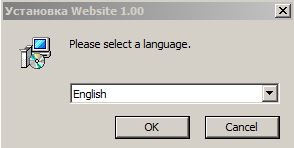
\includegraphics[width=0.7\linewidth]{setuper1}}\\
Первый  шаг установки- выбор языка установки.

\center{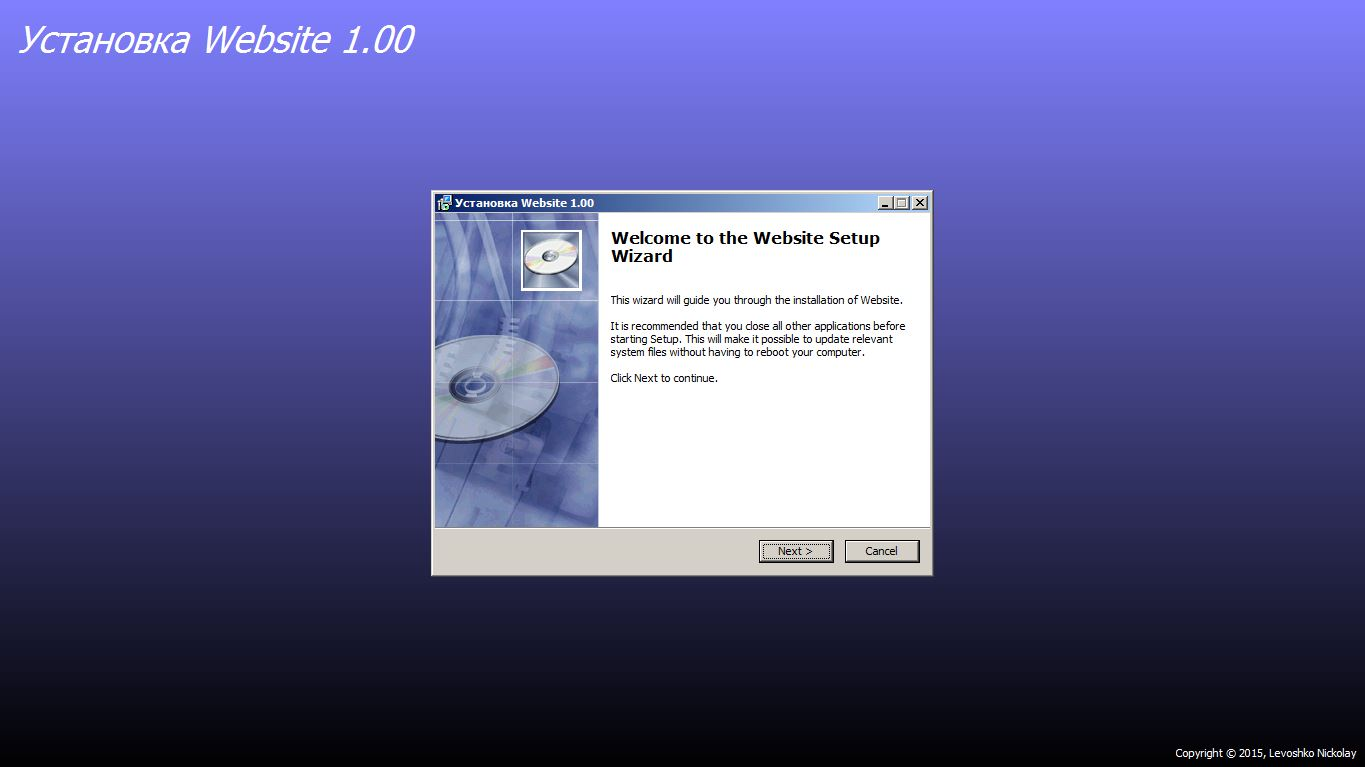
\includegraphics[width=0.7\linewidth]{setuper2}}\\
Второй шаг установки- подтверждение.
\center{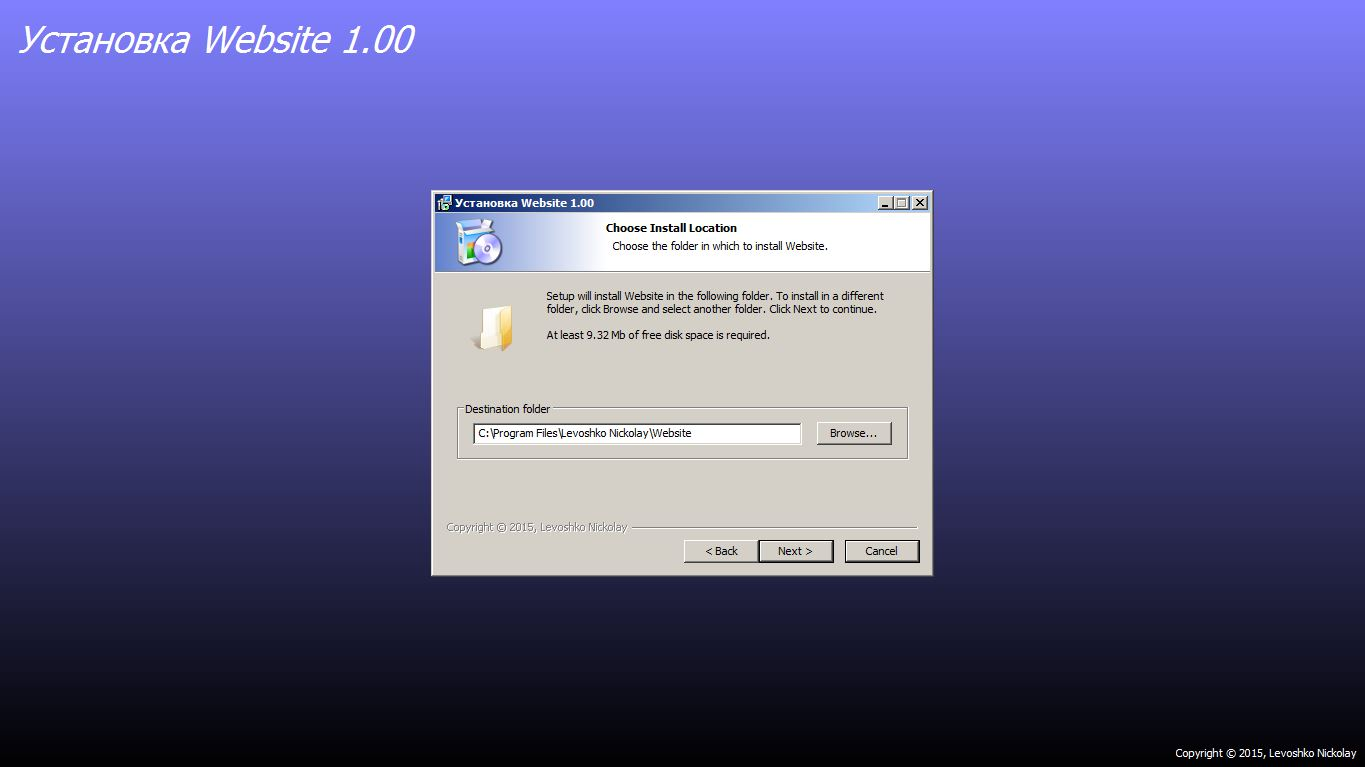
\includegraphics[width=0.7\linewidth]{setuper3}}\\
Третий шаг установки - выбор директории установки.
\center{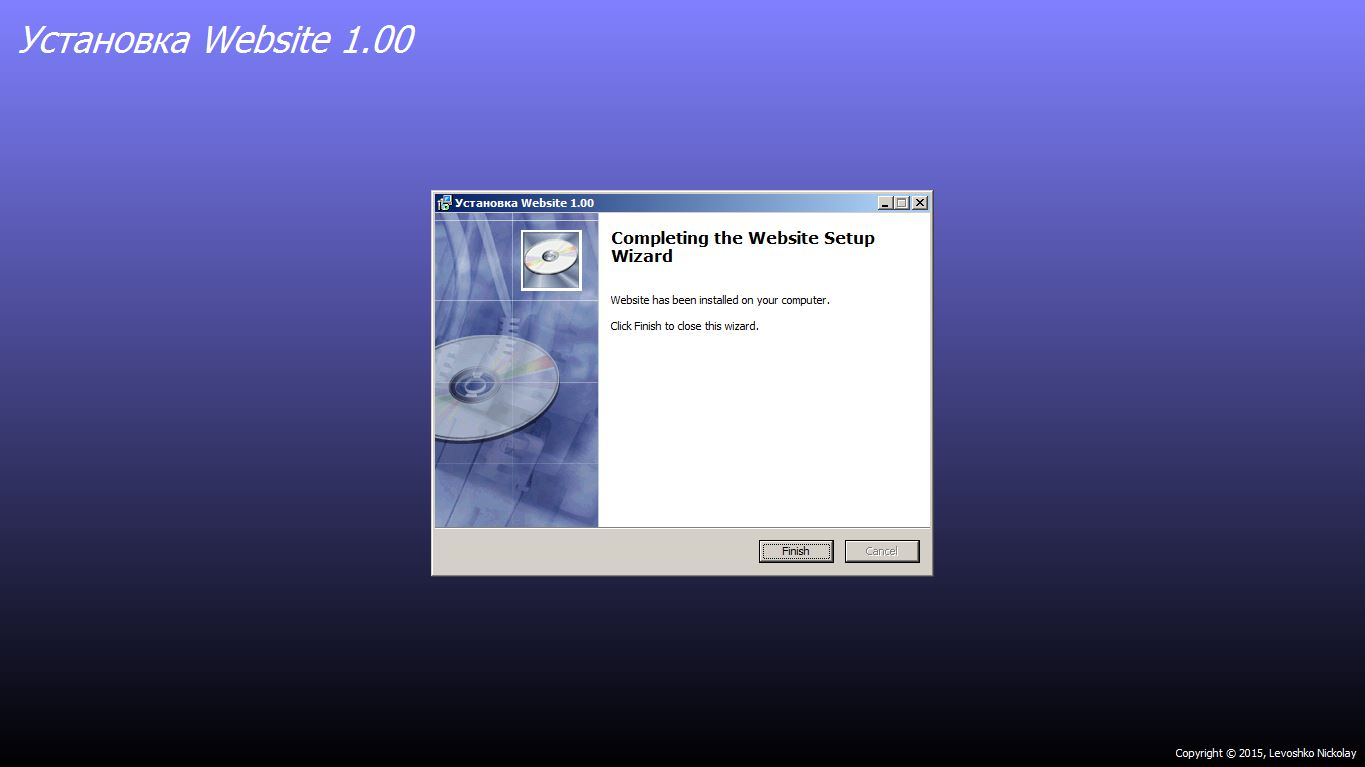
\includegraphics[width=0.7\linewidth]{setuper4}}\\
Последний шаг установки.\\
Приложение готово к использованию.